\documentclass[judge=standard,11pt]{jlreq}

% --- パッケージの読み込み ---
\usepackage{luatexja}
\usepackage{amsmath, amssymb, amsthm}
\usepackage{mathtools}
\usepackage{tikz}
\usepackage{tikz-cd}
\usepackage{tcolorbox}
\usepackage{listings}
\usepackage{xcolor}
\usepackage{hyperref}

% --- TikZの設定 ---
\usetikzlibrary{calc, positioning, arrows.meta, shapes.geometric}

% --- 定理環境の設定 ---
\theoremstyle{definition}
\newtheorem{definition}{定義}[section]
\newtheorem{theorem}[definition]{定理}
\newtheorem{remark}[definition]{注意}
\newtheorem{example}[definition]{例}

% --- マクロ定義 ---
\newcommand{\TowerD}{\mathsf{TowerD}}
\newcommand{\CatD}{\mathsf{Cat\_D}}
\newcommand{\CatLe}{\mathsf{Cat\_le}}
\newcommand{\CatLeExists}{\mathsf{Cat\_le\_exists}}
\newcommand{\CatLeBij}{\mathsf{Cat\_LeBij}}
\newcommand{\CatWithMin}{\mathsf{Cat\_WithMin}}
\newcommand{\HomD}{\mathrm{Hom}_{\mathsf{D}}}
\newcommand{\HomLe}{\mathrm{Hom}_{\mathsf{le}}}
\newcommand{\HomLeExists}{\mathrm{Hom}_{\mathsf{le}\exists}}
\newcommand{\minLayer}{\operatorname{minLayer}}

% --- Lean言語の定義 (listings用) ---
\lstdefinelanguage{Lean}{
  keywords={def, theorem, lemma, structure, class, instance, where, by, intro, exact, simp, rfl, example, abbrev, open, namespace, end, import, noncomputable},
  keywordstyle=\color{blue}\bfseries,
  ndkeywords={Type, Prop, Set, Monotone},
  ndkeywordstyle=\color{teal}\bfseries,
  identifierstyle=\color{black},
  sensitive=true,
  comment=[l]{--},
  morecomment=[s]{/-}{-/},
  commentstyle=\color{green!60!black}\ttfamily,
  stringstyle=\color{purple}\ttfamily,
  morestring=[b]",
}

% --- コード掲載の設定 ---
\lstset{
  language=Lean,
  basicstyle=\ttfamily\small,
  keywordstyle=\color{blue},
  commentstyle=\color{green!60!black},
  stringstyle=\color{purple},
  frame=single,
  breaklines=true,
  columns=fullflexible,
  keepspaces=true,
  showstringspaces=false,
  extendedchars=true,
  % Unicode文字の置換設定
  literate=
    {⟶}{$\longrightarrow$}2
    {→}{$\to$}1
    {∀}{$\forall$}1
    {∃}{$\exists$}1
    {∈}{$\in$}1
    {⊆}{$\subseteq$}1
    {≤}{$\le$}1
    {≥}{$\ge$}1
    {∘}{$\circ$}1
    {𝟙}{$\mathbf{1}$}1
    {≫}{$\gg$}1
    {ℕ}{$\mathbb{N}$}1
    {ℚ}{$\mathbb{Q}$}1
    {ₗₑ}{${}_{\mathrm{le}}$}1
    {ₗₑ∃}{${}_{\mathrm{le}\exists}$}1
    {ₗᵇ}{${}_{\mathrm{le}}^{\mathrm{b}}$}1
    {⥤}{$\rightsquigarrow$}1 % 関手用の記号
}

% --- 文書情報 ---
\title{構造塔の圏論的階層構造：\\Cat\_D, Cat\_le, そして Cat\_eq のランドスケープ}
\author{Lean Code Generation: Codex (OpenAI) \\ TeX Explanation Generation: Gemini (Google)}
\date{\today}

\begin{document}

\maketitle

\begin{abstract}
本稿では、Lean 4によって形式化された「構造塔（Structure Tower）」の多様な圏論的定式化について解説します。
特に、最小層（\texttt{minLayer}）を持たない最も柔軟な圏 \texttt{Cat\_D} から、順序保存を課す \texttt{Cat\_le}、そして \texttt{minLayer} を等式で保存する厳密な圏 \texttt{Cat\_WithMin} までの階層構造を整理します。
各モジュールの設計思想、忘却関手による接続、および「同型射の圏（Groupoid）」と「全単射な射の圏（Bijective lane）」の微妙な差異についても詳述します。
\end{abstract}

\tableofcontents

\section{設計原理と全体図}

構造塔（Structure Tower）の理論は、対象（オブジェクト）の定義と、それらの間の射（モルフィズム）の定義の組み合わせによって複数の「レーン（Lane）」を形成します。
今回の実装では、主に以下の3つの軸で圏が分類されています。

\begin{enumerate}
    \item \textbf{対象の強さ}: \texttt{minLayer} を持つか（\texttt{StructureTowerWithMin}）、持たないか（\texttt{TowerD}）。
    \item \textbf{添字写像のデータ性}: 添字集合間の写像（indexMap）をデータとして持つか（Data）、存在のみを要求するか（Exists）、あるいは全く持たないか。
    \item \textbf{射の強さ}: 層を単に包含関係で保つか、順序を保つか、あるいは \texttt{minLayer} を等式で保存するか。
\end{enumerate}

以下の図は、提供されたファイル群が構成する圏の全体図です。

\begin{figure}[h]
\centering
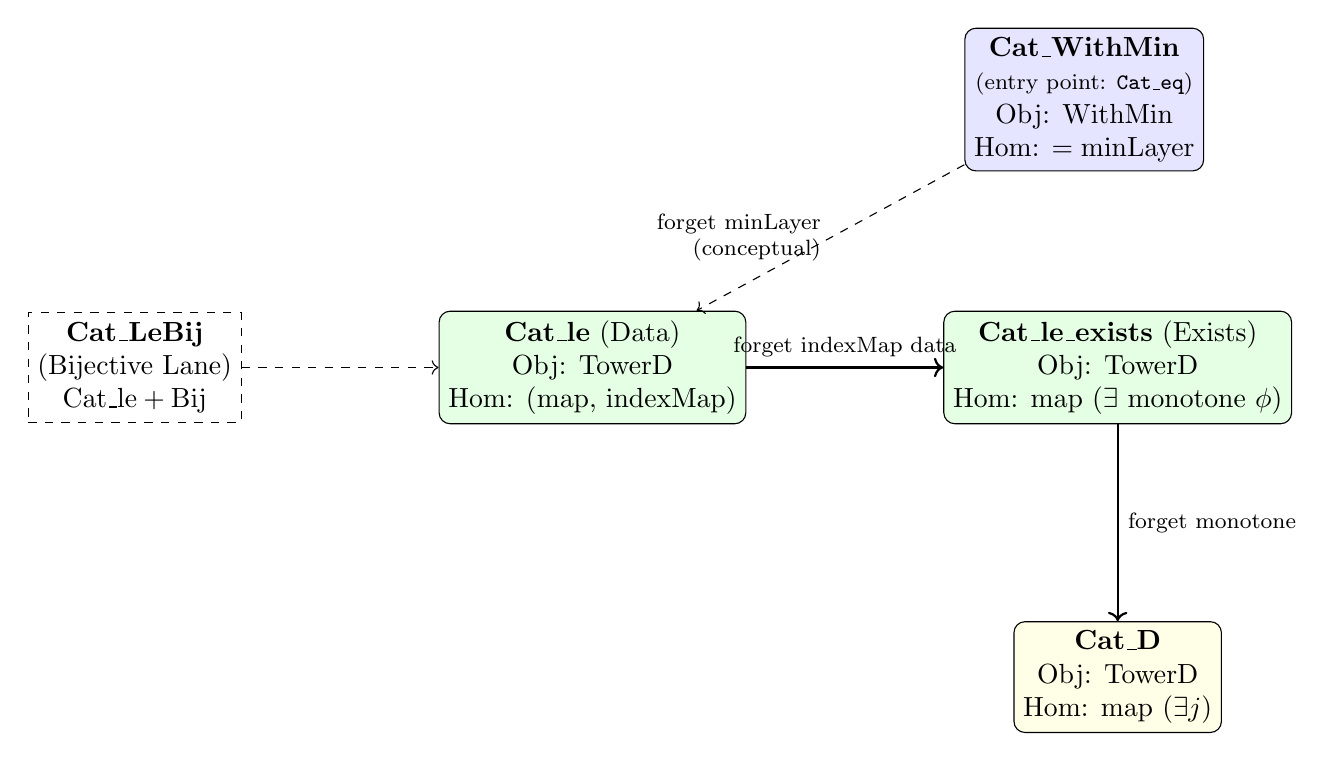
\begin{tikzpicture}[node distance=2.5cm, auto]
    % Nodes
    \node[draw, rectangle, rounded corners, fill=blue!10, align=center] (WithMin) {
        \textbf{Cat\_WithMin}\\
        {\footnotesize (entry point: \texttt{Cat\_eq})}\\
        Obj: WithMin\\
        Hom: $= \minLayer$
    };

    \node[draw, rectangle, rounded corners, fill=green!10, align=center, below left=of WithMin, xshift=-1cm] (Le) {
        \textbf{Cat\_le} (Data)\\
        Obj: TowerD\\
        Hom: (map, indexMap)
    };

    \node[draw, rectangle, rounded corners, fill=green!10, align=center, right=of Le] (LeExists) {
        \textbf{Cat\_le\_exists} (Exists)\\
        Obj: TowerD\\
        Hom: map ($\exists$ monotone $\phi$)
    };

    \node[draw, rectangle, rounded corners, fill=yellow!10, align=center, below=of LeExists] (D) {
        \textbf{Cat\_D}\\
        Obj: TowerD\\
        Hom: map ($\exists j$)
    };

    \node[draw, dashed, align=center, left=of Le] (LeBij) {
        \textbf{Cat\_LeBij}\\
        (Bijective Lane)\\
        $\text{Cat\_le} + \text{Bij}$
    };

    % Arrows (Forgetful functors)
    \draw[->, dashed] (WithMin) -- node[left, font=\footnotesize, align=right] {forget minLayer\\(conceptual)} (Le);
    \draw[->, thick] (Le) -- node[above, font=\footnotesize] {forget indexMap data} (LeExists);
    \draw[->, thick] (LeExists) -- node[right, font=\footnotesize] {forget monotone} (D);
    \draw[->, dashed] (LeBij) -- (Le);

\end{tikzpicture}
\caption{構造塔の圏論的階層図。矢印は忘却関手（情報量の減少）を表す。実線は実装済みの関手、点線は概念的な関係または部分的な実装を示す。}
\end{figure}

\section{Cat\_D}

\texttt{Cat\_D} は、構造塔の理論において最も「薄い（thin）」圏です。
この圏は \texttt{Cat\_D.md} で定義されており、確率論における「フィルトレーション間の可測写像」をモデル化することを主眼としています。

\subsection{対象: TowerD}
対象は \texttt{StructureTower}（別名 \texttt{TowerD}）です。これは \texttt{minLayer} を持たず、単に層の単調増加列 $L_i \subseteq L_j$ ($i \le j$) と被覆性 $\bigcup L_i = X$ を持つ構造です。

\subsection{射: HomD}
射 $\HomD(T, T')$ は、基礎集合間の写像 $f: X \to X'$ のみで構成されます。条件は以下の「存在量化された層保存性」のみです。

\[ \forall i \in I, \exists j \in I', f(L_i) \subseteq L'_j \]

ここには、添字集合間の写像 $\phi: I \to I'$ は明示的に存在しません。「どこかの層に入ればよい」というこの柔軟性は、確率空間の等価性や、異なる時間スケールを持つ過程間の写像を扱う際に有用です。

\section{Cat\_le\_exists (Exists)}

\texttt{Cat\_le\_exists} は、\texttt{Cat\_le} と \texttt{Cat\_D} の中間にある圏です。\texttt{Cat\_le\_exists.md} で定義されています。
これは「存在量化」という点では \texttt{Cat\_D} に近いですが、順序保存性の要請という点では \texttt{Cat\_le} に近い性質を持ちます。

\subsection{動機}
\texttt{Cat\_le} では添字写像 $\phi$ をデータとして持ちますが、場合によっては「適切な順序保存写像 $\phi$ が存在すること」だけを保証し、$\phi$ の具体的な選び方は区別したくないことがあります。

\subsection{射: HomLeExists}
射は $(f, P)$ の対です。ここで $f$ は基礎写像、$P$ は以下の存在命題の証拠です。
\[ \exists \phi: I \to I', \text{Monotone}(\phi) \land (\forall i, f(L_i) \subseteq L'_{\phi(i)}) \]
圏論的には、これは \texttt{Cat\_le} の射から $\phi$ の情報を忘れたものと見なせます。

\section{Cat\_le (data)}

\texttt{Cat\_le} は、順序構造を明示的に保存したい場合の圏です。\texttt{Cat\_le.md} で定義されています。
前の節の \texttt{Cat\_le\_exists} と異なり、ここでは添字写像を**データとして**保持します。

\subsection{射: HomLe}
この圏の射は、データとして $(f, \phi)$ の対を持ちます。
\begin{itemize}
    \item $f: X \to X'$ （基礎写像）
    \item $\phi: I \to I'$ （添字写像）
\end{itemize}

条件として以下が課されます。
\begin{itemize}
    \item $\phi$ は単調増加：$i \le j \implies \phi(i) \le \phi(j)$
    \item 層の保存：$x \in L_i \implies f(x) \in L'_{\phi(i)}$
\end{itemize}

この圏では、同じ写像 $f$ であっても、異なる時間スケール変換 $\phi$ を伴えば「異なる射」として区別されます。

\section{Forgetful functors (Data $\to$ Exists $\to$ D)}

\texttt{Cat\_le\_functors.md} では、これら3つのレーンを繋ぐ忘却関手が定義されています。これらは対象間の単なる写像ではなく、圏から圏への関手（Functor）として実装されています。

\begin{enumerate}
    \item \textbf{forgetIndexMap}: $\CatLe \to \CatLeExists$
    \begin{itemize}
        \item \texttt{Cat\_le} (Data) から \texttt{Cat\_le\_exists} (Exists) へ。
        \item 具体的な $\phi$ を忘れ、その存在性だけを残します。
    \end{itemize}
    
    \item \textbf{forgetToD}: $\CatLeExists \to \CatD$
    \begin{itemize}
        \item \texttt{Cat\_le\_exists} (Exists) から \texttt{Cat\_D} へ。
        \item $\phi$ の「単調性」の要件を忘れ、単に「各層がどこかの層に入る（$\exists j$）」という条件に弱めます。
    \end{itemize}

    \item \textbf{forgetLeToD}: $\CatLe \to \CatD$
    \begin{itemize}
        \item 上記2つの合成です。
    \end{itemize}
\end{enumerate}

なお、型クラスの衝突を避けるため、各圏の対象には \texttt{TowerD\_D}, \texttt{TowerD\_LeExists} といったラッパー型（付録A参照）が使用されています。

\section{Cat\_LeBij（注意：逆が層保存とは限らない）}

\texttt{Cat\_LeBij.md} は、\texttt{Cat\_le} の射に「全単射（Bijective）」という条件を加えた圏を定義しています。

\subsection{定義}
射は \texttt{HomLe} であり、かつ以下の条件を満たすものです。
\begin{itemize}
    \item $f: X \to X'$ が全単射。
    \item $\phi: I \to I'$ が全単射。
\end{itemize}

\subsection{重要：Groupoid ではない}
この圏は「同型射の圏（Groupoid）」ではありません。これは本体系の整理における核心的な注意点です。
構造塔の射において、**写像が全単射であっても、その逆写像が層構造を保存するとは限らない**からです。

例えば、密な層構造を持つ塔から疎な層構造を持つ塔への全単射な順序保存写像が存在しても、逆方向は層を飛び越えてしまう可能性があります。
したがって、これは同型射（Isomorphism）を集めたものではなく、単なる「全単射な射のレーン（Bijective lane）」として理解すべきです。

\subsection{実装上の入口：Cat\_TowerD\_Bij}
\texttt{Cat\_TowerD\_Bij.md} は、この \texttt{Cat\_LeBij} へのエイリアスを提供します。

かつてこの概念は \texttt{Cat\_eq} という名前で呼ばれていたことがありましたが、これは誤解を招く名称でした。
\texttt{Cat\_eq} は後述するように「\texttt{minLayer} を等式で保存する」圏のために予約されるべき名前です。
この混乱を避けるため、\texttt{TowerD} 上の全単射レーンは明確に \texttt{Cat\_TowerD\_Bij} と再命名され、\texttt{Cat\_LeBij} の再輸出として位置づけられています。

\section{WithMin (Cat2) と homeq}

\texttt{Cat\_WithMin.md} は、これまでとは異なる「強い」対象 \texttt{StructureTowerWithMin} を扱います。
これは \texttt{CAT2\_complete.lean} で定義されている構造の再輸出です。

\subsection{対象: WithMin}
対象は \texttt{minLayer} 関数を明示的に持ちます。
\[ \minLayer: X \to I \]
これは各要素 $x$ が属する「最小の」層を一意に指定します。

\subsection{射: homeq}
ここでの射（\texttt{homeq}）は、\texttt{minLayer} を等式で保存することを要求します。
\[ \minLayer(f(x)) = \phi(\minLayer(x)) \]
これは非常に強い条件であり、代数的な普遍性（自由対象など）を議論する際に必須となります。

\section{Cat\_eq}

\texttt{Cat\_eq.md} は現在、\texttt{Cat\_WithMin} へのエイリアス（入口）として固定されています。
これは「等式（Equality）」で構造を保存する、という意味で \texttt{Cat\_eq} という名前が最もふさわしいのが、この \texttt{WithMin} レーンだからです。

\appendix

\section{型ラッパ一覧}

Leanの型クラス推論（Typeclass Inference）において、同一の型（\texttt{TowerD}）に対して複数の異なる \texttt{Category} インスタンスを定義することはできません。
これを回避するため、各ファイルでは以下のようなラッパー型（Type Wrapper）を導入してインスタンスを分離しています。

\begin{itemize}
    \item \textbf{\texttt{TowerD\_D}}: \texttt{Cat\_D.md} で使用。射は \texttt{HomD}（mapのみ）。
    \item \textbf{\texttt{TowerD\_LeExists}}: \texttt{Cat\_le\_exists.md} で使用。射は \texttt{HomLeExists}（map + 存在証明）。
    \item \textbf{\texttt{TowerD\_LeBij}}: \texttt{Cat\_LeBij.md} で使用。射は \texttt{HomLeBij}（全単射な \texttt{HomLe}）。
    \item \textbf{\texttt{TowerD}} (raw): \texttt{Cat\_le.md} ではラッパーなしで直接インスタンス化されている（Dataレーンがデフォルト扱い）。
\end{itemize}

\section{Sanity check 集}

各ファイルには、定義が意図通りであることを確認するための簡単なテスト（Sanity check）が含まれています。これらはすべて \texttt{rfl}（反射性）で証明が完了する単純なものです。

\begin{lstlisting}
-- Cat_WithMin.md
example (T T' T'' : TowerWithMin) (f : T ⟶ T') (g : T' ⟶ T'') :
    (f ≫ g).map = g.map ∘ f.map := rfl

-- Cat_le_functors.md
example (T : TowerD) (x : T.carrier) :
    (forgetLeToD.map (𝟙 T)).map x = x := rfl

-- Cat_le_exists.md
example (T : TowerD_LeExists) (x : (T : TowerD).carrier) :
    (𝟙 T : T ⟶ T).map x = x := rfl

-- Cat_TowerD_Bij.md
example {T T' : TowerD_Bij} (f : T ⟶ T') (x : (T : TowerD).carrier) :
    (ST.Functors.forgetToLe.map f).map x = f.map x := rfl
\end{lstlisting}

\end{document}